%%%%%%%%%%%%%%%%%%%%%%%%%%%%%%%%%%%%%%%%%
% Stylish Article
% LaTeX Template
% Version 2.1 (1/10/15)
%
% This template has been downloaded from:
% http://www.LaTeXTemplates.com
%
% Original author:
% Mathias Legrand (legrand.mathias@gmail.com) 
% With extensive modifications by:
% Vel (vel@latextemplates.com)
% Final ACS by:
% Juan Barbosa
% License:
% CC BY-NC-SA 3.0 (http://creativecommons.org/licenses/by-nc-sa/3.0/)
%
%%%%%%%%%%%%%%%%%%%%%%%%%%%%%%%%%%%%%%%%%
\documentclass[fleqn,10pt]{SelfArx}
%\usepackage[superscript]{cite}
\usepackage{wrapfig}
%----------------------------------------------------------------------------------------
%	ARTICLE INFORMATION
%----------------------------------------------------------------------------------------

\JournalInfo{Laboratorio Avanzado, No. 1, 20/4/2017} % Journal information
\Archive{ }

\PaperTitle{S\'intesis de Dilantin un antiepileptico a partir de benzaldehido} %
%\Keywords{Keyword1 --- Keyword2 --- Keyword3} % Keywords - if you don't want any simply remove all the text between the curly brackets
%\newcommand{\keywordname}{Keywords} % Defines the keywords heading name

%----------------------------------------------------------------------------------------
%	ABSTRACT
%----------------------------------------------------------------------------------------

\Abstract{
\begin{wrapfigure}{r}{0.45\textwidth}
\centering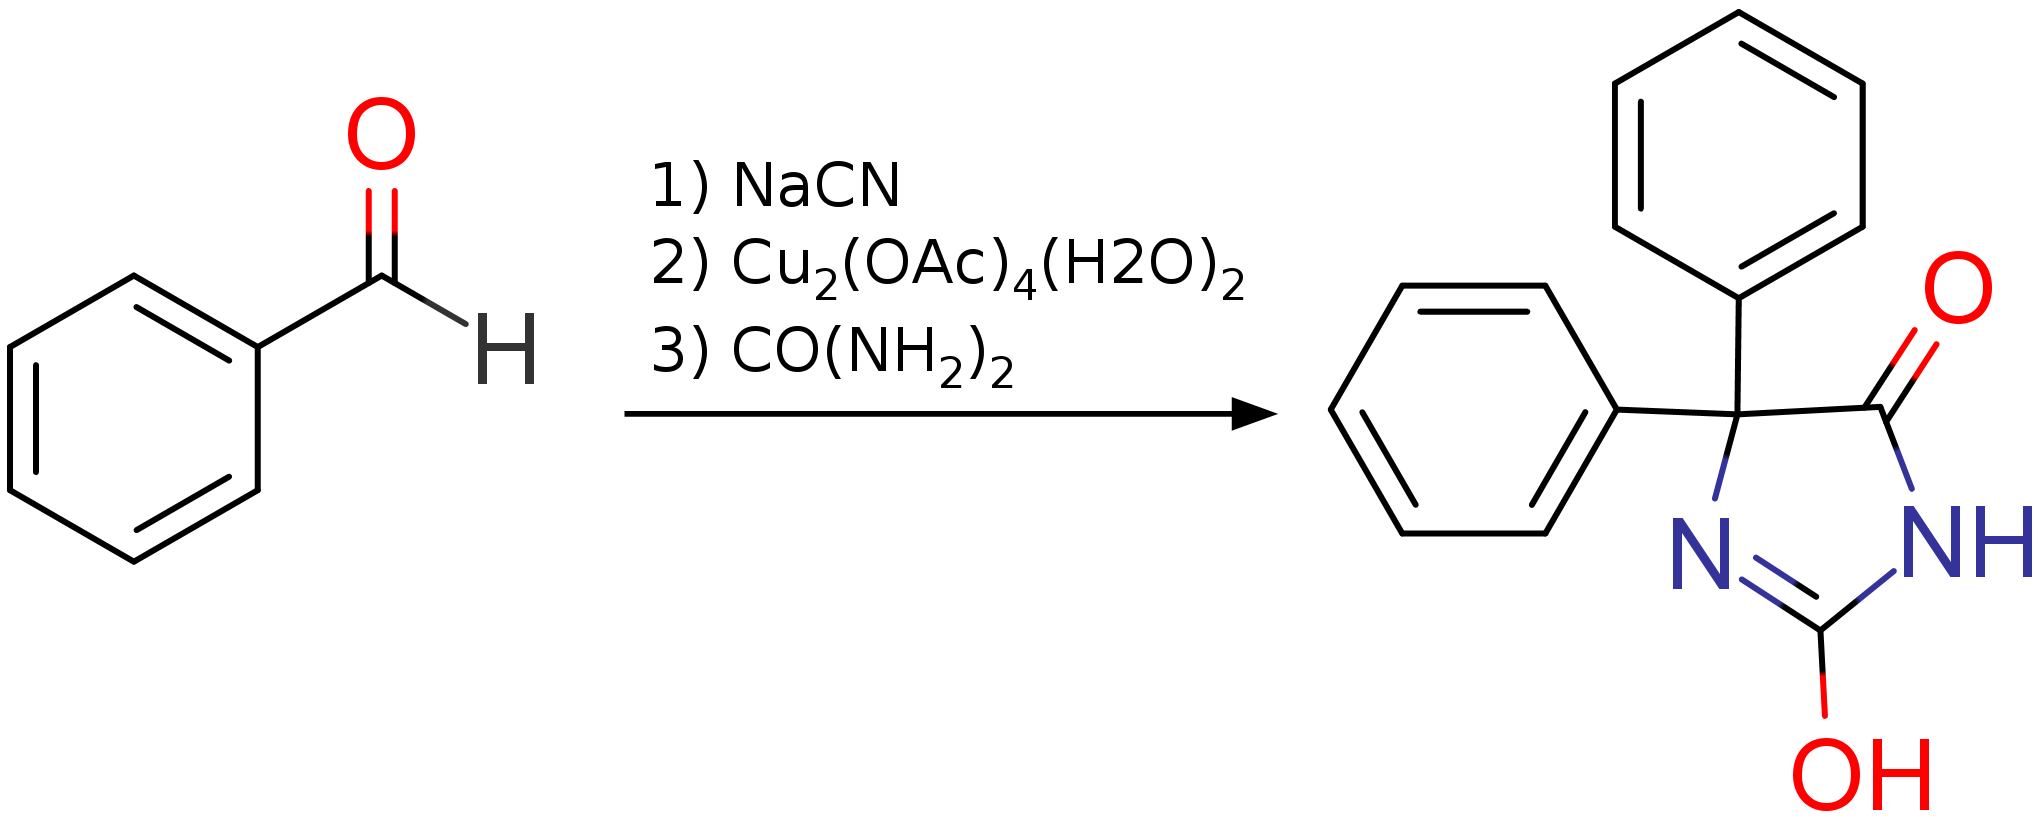
\includegraphics[scale=1]{structures/overall.png}
\end{wrapfigure}
La s\'intesis de la 5,5-difenilimidazolidina-2,4-diona (\textit{Dilantin}) se realiza en 3 etapas a partir del benzaldeh\'ido. El primero corresponde con una condensaci\'on benzo\'inica, el segundo es la oxidaci\'on de la benzo\'ina y finalmente se lleva a cabo un rearreglo benz\'ilico para dar origen al compuesto hidanto\'inico. Las \'ultimas dos etapas son realizadas con dos metodolog\'ias distintas, la primera novedosa y la segunda cl\'asica, usando cerca de la mitad de la benzo\'ina sintentizada cada una. Los rendimientos obtenidos por las dos rutas son \_\_\_\% y \_\_\_\% correspondientemente. Siendo la ruta cl\'asica m\'as apropiada en t\'erminos de rendimiento y pureza, sin embargo la m\'as demandante en tiempo. Se presentan los mecanismos de las distintas etapas de la reacci\'on y su respectivo an\'alisis.
}

%----------------------------------------------------------------------------------------

\begin{document}

\flushbottom % Makes all text pages the same height

\maketitle % Print the title and abstract box

%\tableofcontents % Print the contents section

\thispagestyle{empty} % Removes page numbering from the first page



%----------------------------------------------------------------------------------------
%	ARTICLE CONTENTS
%----------------------------------------------------------------------------------------

\section*{Introducci\'on} % The \section*{} command stops section numbering
Los compuestos de la familia de las hindanto\'inas son importantes medicamentos debido a su alta actividad biol\'ogica en el sistema nervioso central. A pesar que su principal uso es como antiepil\'eptico, tambi\'en es ampliamente usado como agente antiarr\'itmico, antitumor, bactericida y fungicida \cite{safari2010}\cite{ildiz2012}\cite{hayward1983}.
\begin{scheme}[h]
	\centering
	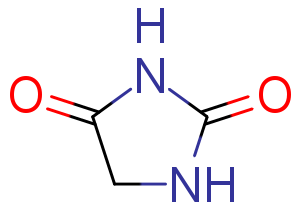
\includegraphics[width=0.3\linewidth]{structures/hydantoin.png}
	\caption{Anillo de hidanto\'ina.}
\end{scheme}

La primera s\'intesis de la 5,5-difenilimidazolidina-2,4-diona (\textit{Dilantin}) fue en 1908 por el qu\'imico aleman Heinrich Biltz, el cual trabaj\'o con varias hindanto\'inas \cite{hayward1983}\cite{aicardi2007}. Desde entonces se han propuesto distintos m\'etodos de s\'intesis entre los cuales se encuentran: en fase s\'olida, one-pot, en pasos m\'ultiples y asistido por ultrasonido \cite{safari2010}. La ruta sint\'etica usada comercialmente es el tratamiento de benzofenona con cianuro de potasio acuoso y carbonato de amonio \cite{hayward1983}. El procedimiento experimental usado en la presente s\'intesis fue realizado en tres pasos divididos en la s\'intesis de la benzo\'ina, la oxidaci\'on de la misma para obtener benzil, y finalmente el rearreglo benz\'ilico.

\newpage

La obtenci\'on de la benzo\'ina se realiz\'o con una condensaci\'on benzo\'inica en presencia de cianuro de sodio. La oxidaci\'on de la misma se llev\'o a cabo usando dos m\'etodos distintos, el primero propuesto por Depreux \cite{depreux1988} en donde el cobre act\'ua como catalizador de la reacci\'on, y el segundo donde se usa \'acido n\'itrico. El \'ultimo paso de la reacci\'on usa los mismos reactivos para ambos m\'etodos, con la diferencia que el primero es asistido por ultrasonido y el segundo se lleva a cabo en reflujo \cite{safari2010}.
\begin{scheme}[h]
	\centering
	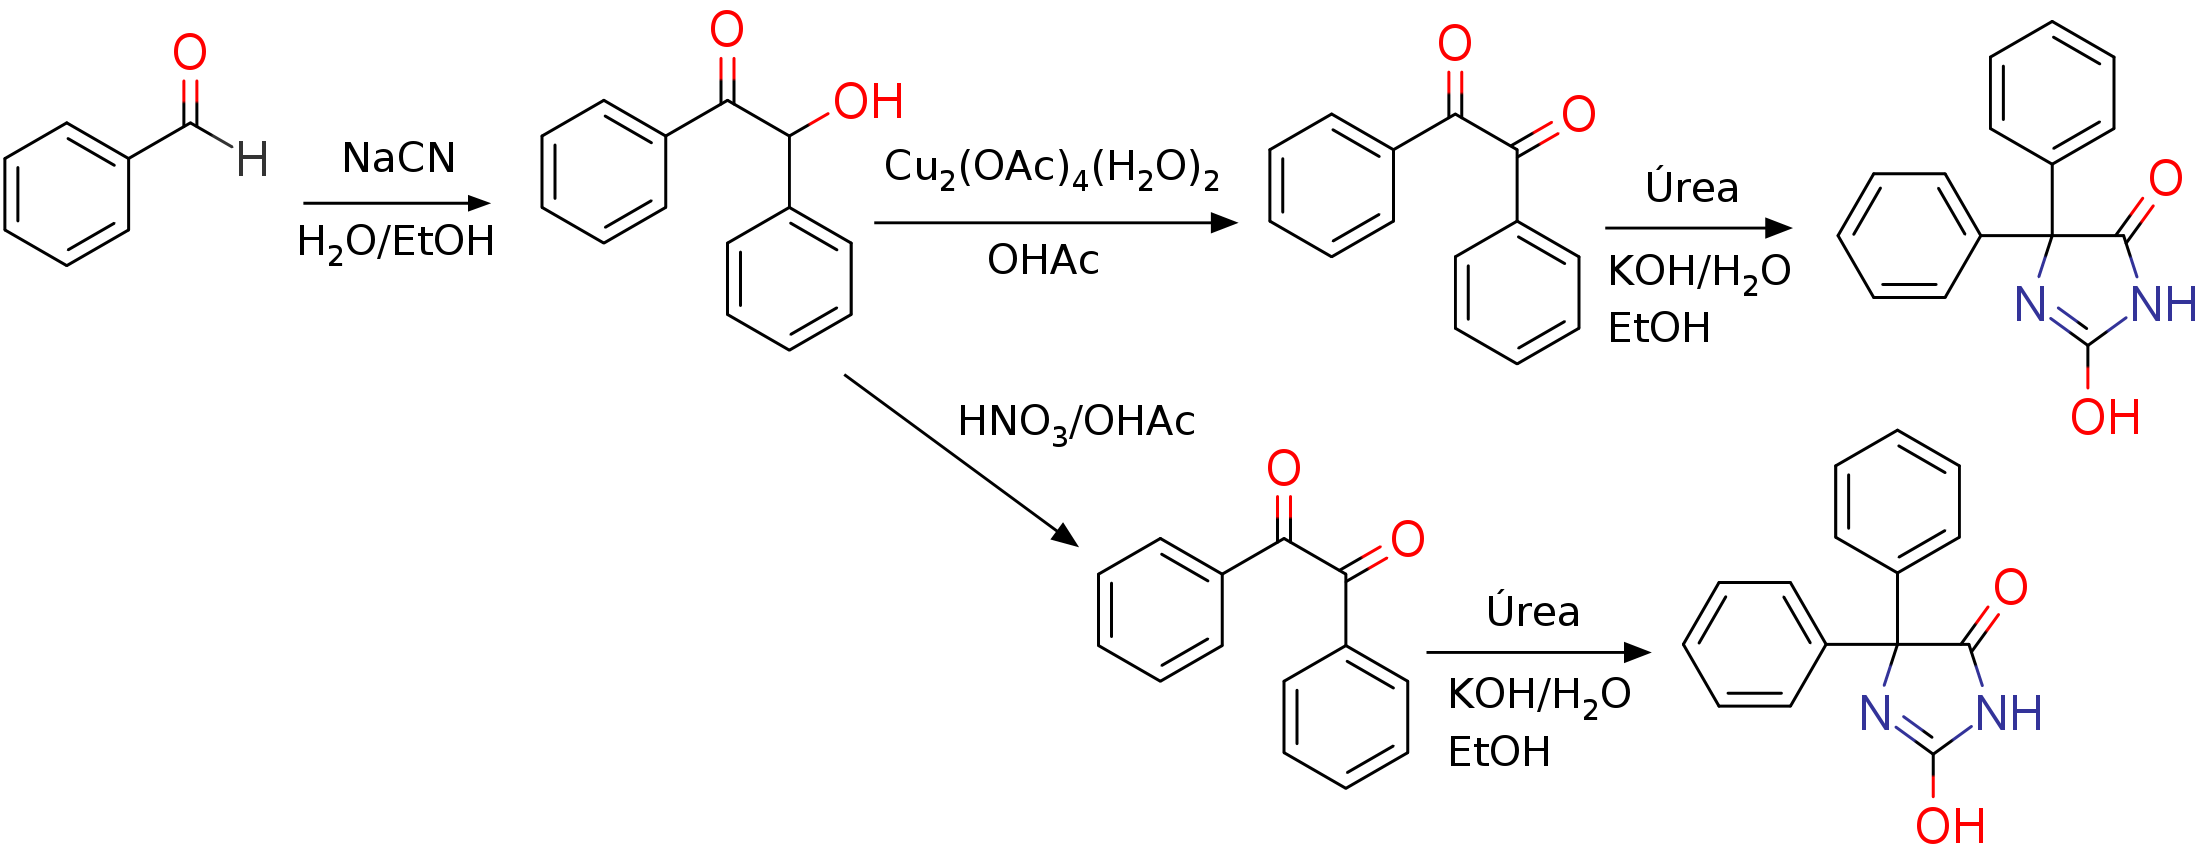
\includegraphics[width=\linewidth]{structures/complete.png}
	\caption{S\'intesis del Dilantin con las dos rutas seguidas en el laboratorio.}
\end{scheme}

%------------------------------------------------

\newpage
\section{Resultados y Discusi\'on}
\section{Conclusiones}
\section{Secci\'on experimental}
Para la elucidaci\'on estructural de los productos se usa informaci\'on espectrosc\'opica de resonancia magn\'etica nuclear prot\'onica de 400 MHz proveniente de un RMN Bruker \_\_\_. El tetrametilsilano es usado como referencia interna, y cloroformo deuterado como solvente para todas las muestras. Adicionalmente se usan los puntos de fusi\'on de los productos obtenidos.

\subsection{S\'intesis de benzoina}
En bal\'on de reacci\'on fueron adicionados 7.0 mL de benzaldeh\'ido sin destilar (68.6 mmol), junto con 6.5 mL de etanol absoluto y 5.0 mL de una soluci\'on acuosa de cianuro de sodio 2.0 M. Una trampa de bicarbonato de sodio en soluci\'on es usada para evitar la protonaci\'on del cianuro. La reacci\'on se lleva a reflujo por 40 minutos. El producto es filtrado y recristalizado en 65 mL de etanol.


\subsection{Oxidaci\'on con acetato de cobre}
La oxidaci\'on de la benzo\'ina se lleva a cabo usando 1.5004 g de acetato de cobre en 8.0 mL de una soluci\'on \'acido ac\'etico y agua (3/1 v/v). Los reactivos se agregan al bal\'on de reacci\'on y se lleva a reflujo en dos etapas de 20 minutos cada una. El producto se filtra y se purifica por columna usando fase movil \_\_\_ : \_\_\_.

\subsection{Oxidaci\'on con \'acido n\'itrico}
Una soluci\'on de 4.3 mL de \'acido ac\'etico en 6.4 mL de \'acido n\'itrico se adiciona a un bal\'on de reacci\'on con 0.846 g de benzo\'ina. El mismo se lleva a reflujo con una trampa de bicarbonato. La reacci\'on tiene una duraci\'on de 2 horas y 30 minutos. Posterior a este tiempo se enfr\'ia la soluci\'on y se agregan 50 mL de agua fr\'ia y se agita hasta la formaci\'on de cristales. El producto se filtra al vac\'io y se seca en horno.

\subsection{S\'intesis de Dilant\'in asistido por ultrasonido}
En un tubo de ensayo se adicionan 0.228 g de \'urea junto con 0.688 g de benzil. Los s\'olidos se disuelven en 5.0 mL de etanol absoluto. Posteriormente se adicionan \_\_\_ mL de una soluci\'on 0.57 M de hidr\'oxido de potasio. La reacci\'on se lleva a cabo en un sonicador a temperatura ambiente por 20 minutos. Una semana despu\'es se acidifica el producto con \'acido clorh\'idrico concentrado, con la adici\'on de agua se da la formaci\'on de precipitado. El mismo es filtrado al vac\'io y secado en horno. 
%----------------------------------------------------------------------------------------
%	REFERENCE LIST
%----------------------------------------------------------------------------------------
\phantomsection
\bibliography{informe}
\bibliographystyle{unsrt}

%----------------------------------------------------------------------------------------
\newpage
\onecolumn
\section{Informaci\'on de soporte}
\begin{figure*}[ht]
	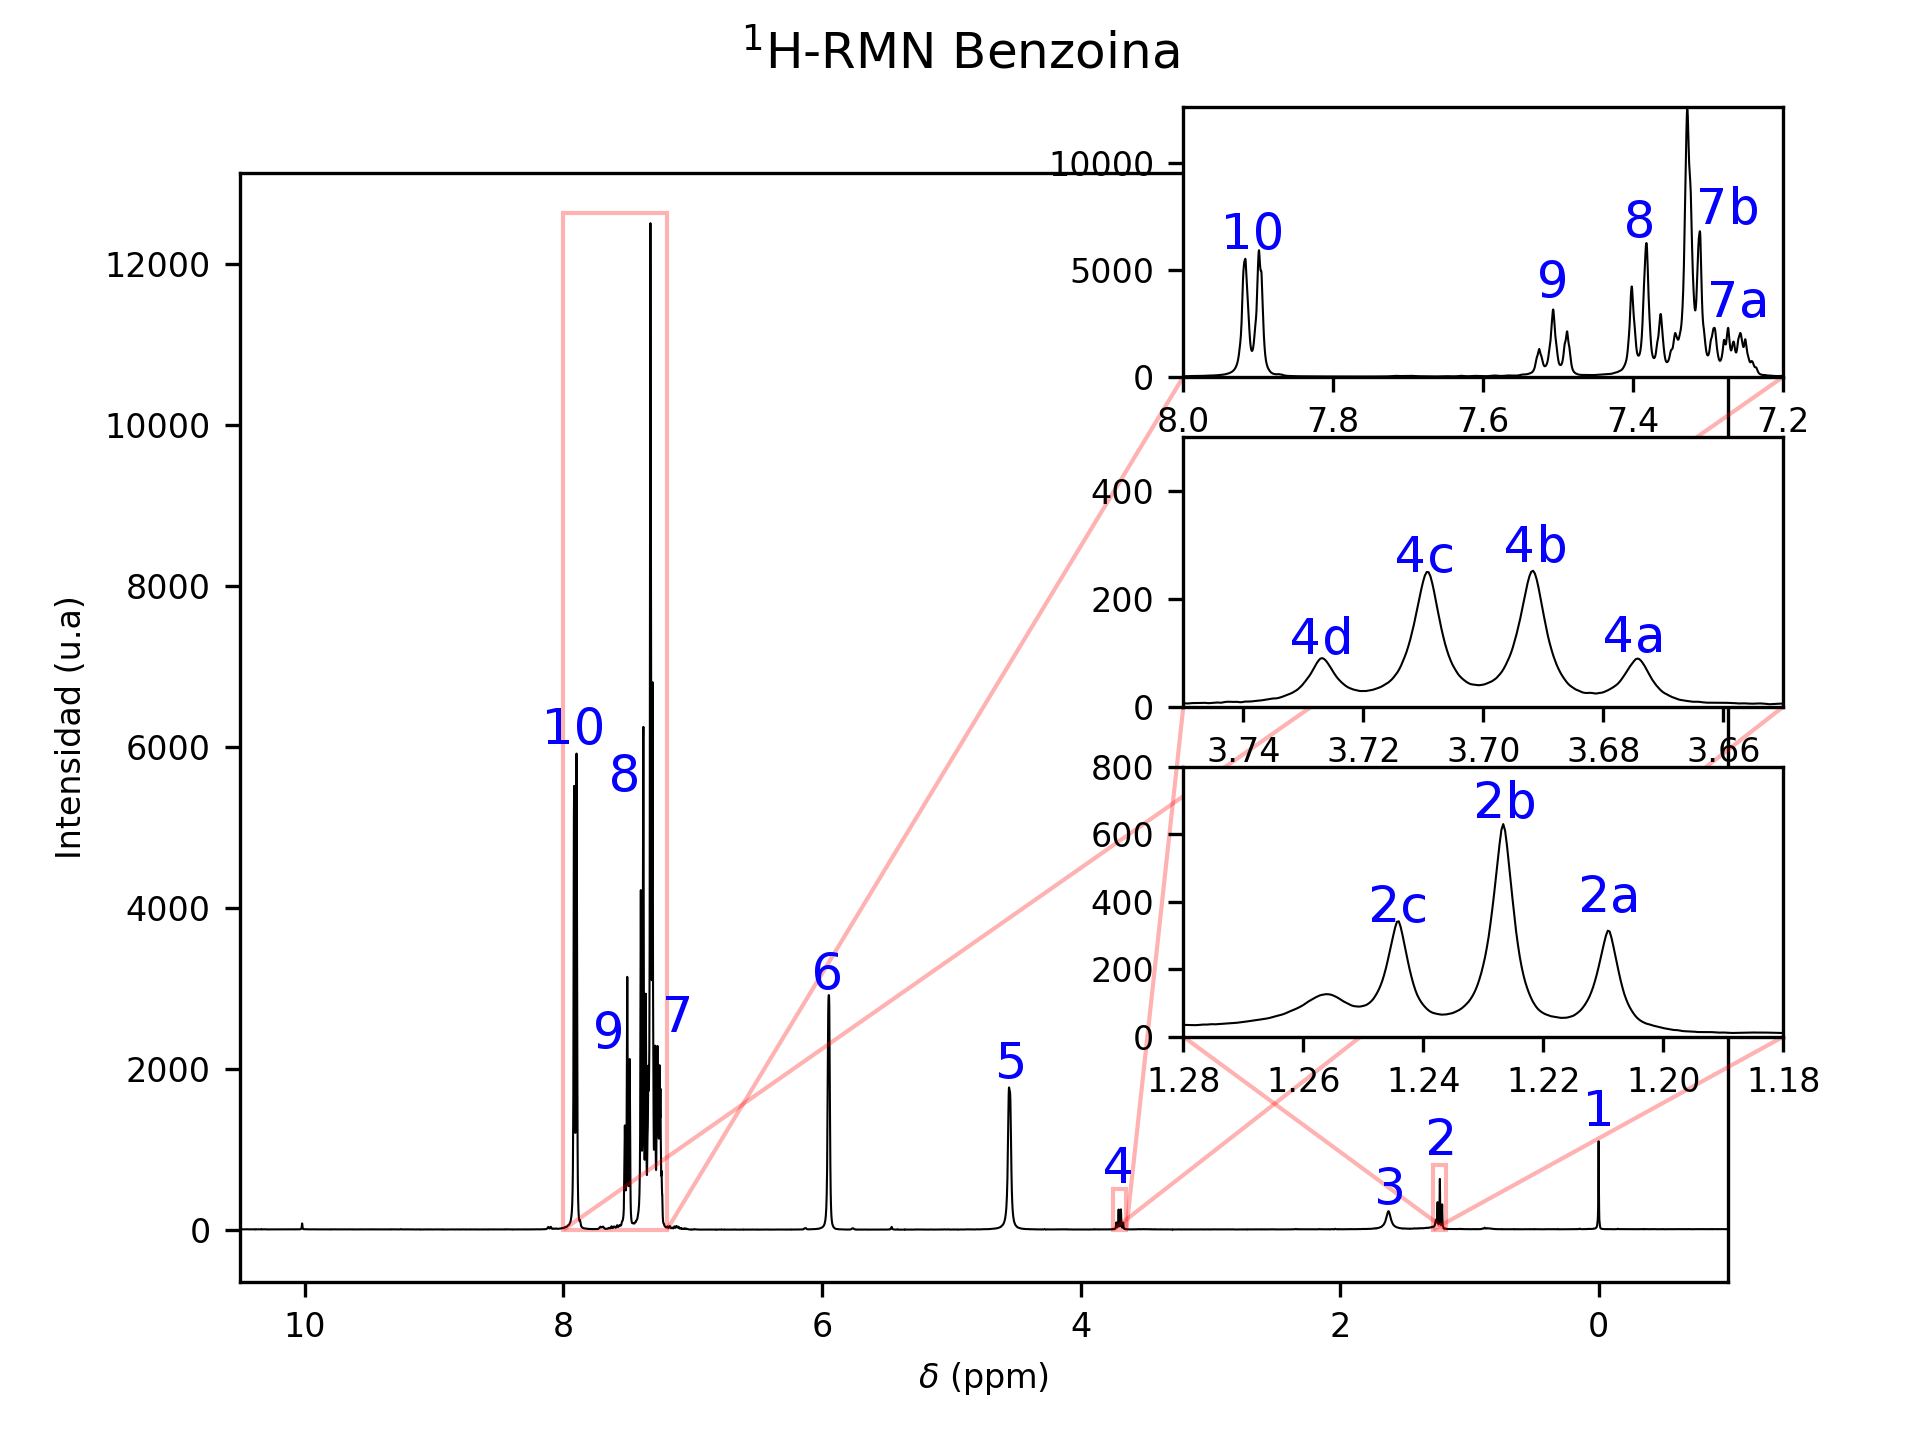
\includegraphics[width=\linewidth]{data/H-Benzoina-edited.png}
\end{figure*}
\end{document}